\def\year{2020}\relax
%File: formatting-instruction.tex
\documentclass[letterpaper]{article} % DO NOT CHANGE THIS
\usepackage{aaai20}  % DO NOT CHANGE THIS
\usepackage{times}  % DO NOT CHANGE THIS
\usepackage{helvet} % DO NOT CHANGE THIS
\usepackage{courier}  % DO NOT CHANGE THIS
\usepackage[hyphens]{url}  % DO NOT CHANGE THIS
\usepackage{graphicx} % DO NOT CHANGE THIS
\usepackage{algorithm,algorithmic}
\usepackage{amsmath,amssymb,amsfonts}
\usepackage{subcaption}
\captionsetup{compatibility=false}
\urlstyle{rm} % DO NOT CHANGE THIS
\def\UrlFont{\rm}  % DO NOT CHANGE THIS
\usepackage{graphicx}  % DO NOT CHANGE THIS
\frenchspacing  % DO NOT CHANGE THIS
\setlength{\pdfpagewidth}{8.5in}  % DO NOT CHANGE THIS
\setlength{\pdfpageheight}{11in}  % DO NOT CHANGE THIS
%\nocopyright
%PDF Info Is REQUIRED.
% For /Author, add all authors within the parentheses, separated by commas. No accents or commands.
% For /Title, add Title in Mixed Case. No accents or commands. Retain the parentheses.
\pdfinfo{
/Title (Hybridization of GRASP algorithm with genetic algorithm.)
/Author (Christian Perez, Miguel A. Salido)
%/Author (Christian Perez, Miguel A. Salido, David Gurrea)
} %Leave this	
% /Title ()
% Put your actual complete title (no codes, scripts, shortcuts, or LaTeX commands) within the parentheses in mixed case
% Leave the space between \Title and the beginning parenthesis alone
% /Author ()
% Put your actual complete list of authors (no codes, scripts, shortcuts, or LaTeX commands) within the parentheses in mixed case.
% Each author should be only by a comma. If the name contains accents, remove them. If there are any LaTeX commands,
% remove them.

% DISALLOWED PACKAGES
% \usepackage{authblk} -- This package is specifically forbidden
% \usepackage{balance} -- This package is specifically forbidden
% \usepackage{caption} -- This package is specifically forbidden
% \usepackage{color (if used in text)
% \usepackage{CJK} -- This package is specifically forbidden
% \usepackage{float} -- This package is specifically forbidden
% \usepackage{flushend} -- This package is specifically forbidden
% \usepackage{fontenc} -- This package is specifically forbidden
% \usepackage{fullpage} -- This package is specifically forbidden
% \usepackage{geometry} -- This package is specifically forbidden
% \usepackage{grffile} -- This package is specifically forbidden
% \usepackage{hyperref} -- This package is specifically forbidden
% \usepackage{navigator} -- This package is specifically forbidden
% (or any other package that embeds links such as navigator or hyperref)
% \indentfirst} -- This package is specifically forbidden
% \layout} -- This package is specifically forbidden
% \multicol} -- This package is specifically forbidden
% \nameref} -- This package is specifically forbidden
% \natbib} -- This package is specifically forbidden -- use the following workaround:
% \usepackage{savetrees} -- This package is specifically forbidden
% \usepackage{setspace} -- This package is specifically forbidden
% \usepackage{stfloats} -- This package is specifically forbidden
% \usepackage{tabu} -- This package is specifically forbidden
% \usepackage{titlesec} -- This package is specifically forbidden
% \usepackage{tocbibind} -- This package is specifically forbidden
% \usepackage{ulem} -- This package is specifically forbidden
% \usepackage{wrapfig} -- This package is specifically forbidden
% DISALLOWED COMMANDS
% \nocopyright -- Your paper will not be published if you use this command
% \addtolength -- This command may not be used
% \balance -- This command may not be used
% \baselinestretch -- Your paper will not be published if you use this command
% \clearpage -- No page breaks of any kind may be used for the final version of your paper
% \columnsep -- This command may not be used
% \newpage -- No page breaks of any kind may be used for the final version of your paper
% \pagebreak -- No page breaks of any kind may be used for the final version of your paperr
% \pagestyle -- This command may not be used
% \tiny -- This is not an acceptable font size.
% \vspace{- -- No negative value may be used in proximity of a caption, figure, table, section, subsection, subsubsection, or reference
% \vskip{- -- No negative value may be used to alter spacing above or below a caption, figure, table, section, subsection, subsubsection, or reference

\setcounter{secnumdepth}{0} %May be changed to 1 or 2 if section numbers are desired.

% The file aaai20.sty is the style file for AAAI Press
% proceedings, working notes, and technical reports.
%
\setlength\titlebox{2.5in} % If your paper contains an overfull \vbox too high warning at the beginning of the document, use this
% command to correct it. You may not alter the value below 2.5 in
\title{Hybridization of GRASP algorithm with genetic algorithm.}
%Your title must be in mixed case, not sentence case.
% That means all verbs (including short verbs like be, is, using,and go),
% nouns, adverbs, adjectives should be capitalized, including both words in hyphenated terms, while
% articles, conjunctions, and prepositions are lower case unless they
% directly follow a colon or long dash
% \author{}
\author{\Large \textbf{Christian Perez, Miguel A. Salido}\\ % All authors must be in the same font size and format. Use \Large and \textbf to achieve this result when breaking a line
\textsuperscript{\rm 1}Universitat Politécnica de Valencia\\
% Institute for Automation and Industrial Computing\\ %If you have multiple authors and multiple affiliations
% use superscripts in text and roman font to identify them. For example, Sunil Issar,\textsuperscript{\rm 2} J. Scott Penberthy\textsuperscript{\rm 3} George Ferguson,\textsuperscript{\rm 4} Hans Guesgen\textsuperscript{\rm 5}. Note that the comma should be placed BEFORE the superscript for optimum readability
Camí de Vera s/n\\
Valencia, Spain\\
cripeber@doctor.upv.es, msalido@dsic.upv.es % email address must be in roman text type, not monospace or sans serif
}
 \begin{document}

 \maketitle


\begin{abstract}
    (Por escribir)
\end{abstract}
\section*{Introduction}

(Por Escribir)


\section*{Problem specification}

This section features the most relevant aspects of the problem specification proposed by the company with the intention of providing a better comprehension of the presented algorithm. The objective of the problem to solve is to minimize the transport cost and the stock cost by assigning each travel to a warehouse, taking into account every characteristic of each travel and warehouse. The minimum cost of transportation is obtained by finding the trip with the minimum value of transportation, which makes this process relatively easy to perform. However, a problem arises when looking for the minimum stock cost due to the fact that there must be a balance between the stock of each type of container. In order to solve this problem, it is needed to stablish a multi-objective function by assigning weights to the stock cost and the transport cost in order to determine the fitness function. The objective of this function is to maintain a stable transport cost while distributing homogeneously the stock between the warehouses. Thus, the most important variables in the problem are taken into account.

\begin{itemize}
  \item \textbf{Transport cost }(TC): Cost asociated with an order and based on the distance between the warehouse and the starting point. This is one of the values that is taken into account in the calculation of the final cost in the fitness function.
  \item \textbf{Stock cost }(SC): If an order is assigned to be loaded at a warehouse where the current stock is less than the stock requested, the negative stock remaining given by this load operation must be replaced. Thus, the cost of the stock is proportional to the product of the cost of replacing each of the items and the negative stock.
  \item \textbf{Delay of delivery }(DD): Each warehouse that can be associated with an order is located in a different place, such that the distance between each warehouse and the starting point is different. Therefore, the delay of delivery value depends on the warehouse chosen by the order. This delay affects how much stock is reduced from the warehouse from the scheduled date to the actual delivery date.
  \item \textbf{Single load point }(SLP): For each order there is a number of possible warehouses where it can be loaded. All the items in an order must be loaded in the same location, creating the constraint that each order can only be loaded at one warehouse.
\end{itemize}

The problem is formed by a dataset (DS) that is based on the combination of three main elements. This three elements contain all of the information necessary to represent an instance of the problem (see Equation \ref{eq:Dataset}). Hence, each problem instance is formed by a group of orders (O) each of which represent a trip to transport items, all of the warehouses that have every item requested by the order (W), and a set of prices (P) for each item. 

\begin{equation}\label{eq:Dataset}
    \begin{aligned}
        DS = \{O, W, P\} \\
    \end{aligned}
\end{equation}
  
The set $O = \{o_1, o_2, \dots, o_N \}$ contains all orders, where $N$ is the number of orders. Each order $o_i \in O$ is formed by three parameters $o_i =[D_{o_i},Ir_{o_i},W_{are_{o_i}}]$:
\begin{itemize}
    \item $D_{o_i}$ is the delivery date of $o_i$.
    \item $Ir_{o_i}$ is the set of items requested in the order $o_i$ (see Equation \ref{eq:OI}). Each element $ir_{o_{i}j} \in Ir_{o_i}$ represents the number of items that have to be loaded.
    \begin{equation}\label{eq:OI}
        \begin{aligned}
            Ir_{o_{i}} = \{ ir_{o_{i}1}, ir_{o_{i}2} \dots, ir_{o_{i}P} \} \\
        \end{aligned}
    \end{equation}
    \item $W_{are{o_i}}$ is the set of possible warehouses that have every item requested in order $o_i$ (see Equation \ref{eq:OW}).
    \begin{equation} \label{eq:OW}
        \begin{aligned}
            Ware_{o_i} = \{ Ware_{o_{i}1}, Ware_{o_{i}2}, \dots Ware_{o_{i}Q} \}\\
        \end{aligned}
    \end{equation}
    Each $W_{o_{i}j}$ is formed by three values:
    \begin{itemize}
        \item $ava_{o_{i}j}$ represents if the warehouse $j$ is available to load all of the items requested by the order $o_i$. Therefore, $ava_{o_{i}j}=1$  means that the warehouse is available, and $ava_{o_{i}j}=0$ means that it is not.
        \item $pr_{o_{i}j}$ contains the transport cost of order $o_i$ from warehouse $j$. If $ava_{o_{i}j}=0$, this value is null.
        \item $dl_{o_{i}j}$ is the delay to load the order $o_i$ from warehouse $j$. If $ava_{o_{i}j}=0$, this value is null.
    \end{itemize}
\end{itemize}

At the beginning of each week and in order to control the amount of stock, the current status of each warehouse is provided by the company through the use of a three-dimensional matrix $W$ (see Equation \ref{eq:W}).
\begin{equation}
    \begin{aligned}\label{eq:W}
        W = \{w_1, w_2, w_3, \dots w_P \}\\
    \end{aligned}
\end{equation}
where each $wst_i \in W$ is composed of a bidirectional matrix (item x week days ). Each of the logistic centers (warehouses) has the ability to replace the lack of items by shipping them. This allows the company to generate negative stock in the warehouses asociated to an order $wst_{ijk} \in \mathbb{N} $.

Finally, $P$ is the set of unitary price for each items (see Equation \ref{eq:P}).

\begin{equation}
    \begin{aligned}\label{eq:P}
        P = \{p_1, p_2, p_3, \dots, p_i, \dots p_P \}\\
    \end{aligned}
\end{equation}


\section*{Solving techniques}

This section explains the different algorithms being used in the evaluation of the solving of the problem proposed by the company, pointing out the the final method used, which is an hybridization of the GRASP algorithm and a Genetic Algorithm (GA). The resolution techniques presented are the Greedy algorithm, the GRASP algorithm and the Genetic Algorithm.

\subsection*{The Greedy algorithm }
Currently, the purpose of the company is to plan orders each week that are based on the demand of customers, considering the expected available stock for each day. The solution for this purpose is based on a greedy technique. The availability of each item is obtained from a given loading plan that its updated each week. This update consists on the stock remaining from the week before, the stock obtained by shipments, etc. This algorithm is determined by different constraints, imposed by factors such as customers, warehouses and geographical areas:

\begin{itemize}
    \item There are clients who only allow loading at specific warehouses due to convenience factors and distance.
    \item The assingments of warehouses to orders have a priority that is dependent on the geographical area or zone of influence.
    \item The order is restricted by the type of items it contains, thus it can not load at a warehouse that does not have every item requested.
    \item Theq quantity of products (vegetables, fruits, fishes) is not constant thorughout the year, therefore the warehouses have different delays for each product depending on the time of the year.
\end{itemize}
The current algorithm developed by the company is composed of two layers. First, the algorithm uses a heuristic called closeness centrality that obtains a measure of centrality of a transport network by adding the distance between the different nodes, obtaining the central nodes (warehouses) as those that have minimum distance to the other nodes. Then, all orders are classified according to the item with the largest part of the order.

In the second layer, if an order does not meet the restrictions of the first layer it is not assigned to a warehouse. These orders are assigned warehouses with larger stock that are less central. The orders that are still unassigned can be reordered using the customers in order to improve the warehouse system or to make up for the lack of stock. However, there may be still unassigned orders which are assigned after an expert human looks for combinations that improve the global transport cost withouth increising stock cost.
It is necessary for an expert to review all of the trips in order to obtain a better solution for the company.

\subsection*{GRASP}

A GRASP algorithm has been developed taking into account the drawbacks of the Greedy algorithm used by the company, in order to obtain in terms of stock balance and travel cost a balanced solution. 

\begin{algorithm}[H]
    \caption{GRASP}
    \label{alg:GRASP}
    \begin{algorithmic}[1] \label{code:grasp}
        \STATE \textit{input: } All orders $O$, All stock matrix $W$, Item price vector $P$, Size of LCR list $n$
        \STATE \textit{output: } Optimized solution $s^*$
        \STATE $i \longleftarrow 0 $
        \STATE $ t \longleftarrow [1,2,3,\dots,|O|]$
        \STATE $LCRordering(\alpha)$\label{LCRordering}
        \STATE
        \STATE $s \longleftarrow [\quad] $
        \STATE $LCR \longleftarrow [o_1,\dots,o_n]$
        \STATE \textbf{while } $|s| \neq |LCR|$ \textbf{do}:\label{1grasp}
        \STATE \quad $j \longleftarrow 0 $
        \STATE \quad $lcr \longleftarrow [\quad]$
        \STATE \quad \textbf{while } $j < |LCR|$ \textbf{do}:
        \STATE \quad \quad $lcr \longleftarrow lcr \cup \textbf{LocalSearch}(LCR_j,\alpha,|LCR|)$
        \STATE \quad \quad $j \longleftarrow j + 1$
        \STATE \quad $\textbf{end while}$
        \STATE \quad $s \longleftarrow s \cup lcr*$ 
        \STATE \quad $LCR \longleftarrow LCR \setminus lcr*$ 
        \STATE \quad $LCR \longleftarrow LCR \cup  o_{n+1} $ 
        \STATE $\textbf{end while}$\label{2grasp}
    \end{algorithmic}
\end{algorithm}


The GRASP Algorithm \ref{code:grasp} is composed of two parts. First, the set of orders is sorted with purpose of improving the efficiency of the algorithm (line \ref{LCRordering}). This type of sorting is based on the idea of constrainedness, meaning giving the algorithm more decision power in the last iterations by analyzing the most restrictive orders in the beginning. Second, in the iterative part of GRASP (from line \ref{1grasp} to \ref{2grasp}), a list (called LCR) that contains the candidates to assign a warehouse given by the algorithm is obtained. Later, through the use of local search the best warehouse stablished. When the best warehouses for all the trips are known, the warehouse with the lowest cost is selected, deleting the order from the LCR list and adding the next one.

\subsubsection*{LRC ordering:}
In order to provide more flexibility and to test the algorithm with different data inputs, the LCR list is sorted. This ordering consists in different steps. First as a pre-processing, every order that only has one available warehouse due to restrictions and availability is automatically allocated. Second, the order of the list is based on the number of possible warehouses, positioning in the first order the trips with fewer possible warehouses, allowing the algorithm to employ less decisions in this assignations. The trips with the same number of warehouses are sorted by the number of items requested by each trip, positioning the ones with fewer items first.



\subsection*{Local search}
With the LCR list sorted, a local search is executed with the intention of obtaining the best assignation. This is performed by obtaining the objetive function for each warehouse in a trip. This function consists on the calculation of the transport cost and the stock cost, giving more weight to the transport cost by means of a parameter called alpha, because the transport generates more costs.

\begin{algorithm}[H] \label{code:LocalSearch}
    \caption{Local Search}
    \begin{algorithmic}[1]
        \STATE \textit{input: } A order $o$, List of item price $P$, Alpha value for objective function $\alpha$, Length of LCR list $nLCR$
        \STATE \textit{output: } Index of warehouse chosen $j$, Minimum cost of warehouse chosen $Q*$
        \STATE  $Q \longleftarrow [\quad]$
        \STATE  $I \longleftarrow Ir_{o}$
        \STATE  $M \longleftarrow W_{o}$
        \STATE  \textbf{For} $j$ \textbf{in} $\{ 0,\dots,|M|\}$:
        \STATE  \quad $Cs \longleftarrow []$
        \STATE  \quad $Ct \longleftarrow \textbf{getTransportCost}(M_j) $ \label{eq:ct}
        \STATE  \quad \textbf{For} $i$ \textbf{in} $\{ 0,\dots,|I|\}$:
        \STATE  \quad \quad $Cs_i \longleftarrow P_i * \sum_{k=D_{o}}^{|wst_{ij}|} wst_{ijk}\; |\; wst_{ijk} < 0 $ 
        \STATE  \quad \quad$Cs \longleftarrow Cs \cup Cs_i $ \label{eq:cs}
        \STATE  \quad  $\textbf{end for}$
        \STATE  \quad $Q_j \longleftarrow \alpha * Ct + (1 - \alpha) * \sum Cs$ \label{eq:fitness}
        \STATE  \quad $Q \longleftarrow Q \cup Q_j$ \label{eq:fitness}
        \STATE  \quad $F_{\alpha}  \longleftarrow (1-\alpha) / nLCR$ \label{eq:fitness}
        \STATE  \quad \textbf{if} $\sum Cs < 0$ \textbf{then}:
        \STATE  \quad \quad $\alpha \longleftarrow \alpha + F_{\alpha}$
        \STATE  \quad $\textbf{else:}$
        \STATE  \quad \quad $\alpha \longleftarrow \alpha - F_{\alpha}$
        \STATE  \quad $\textbf{end if}$
        \STATE  $\textbf{end for}$
    \end{algorithmic}
\end{algorithm}


The transport cost is calculated by the addition of the price of traveling to a warehouse for each order. The stock cost is calculated by the subtraction of the quantity of an item required by a warehouse at a certain time, and then multiplying the cost of manufacturing this item if the quantity remaining is negative. If the stock is positive, the cost will be zero. Finally the warehouse that provides a better value of the obtjective function is chosen.

\subsection*{Improvements}
There have appeared several problems regarding the optimization of the solution during the developement of the algorithm, in order to resolve them, some sections of the code have been imiproved:
\begin{itemize}
    \item \textbf{LCR sorting:} ADesgranstics, there have been a sorting of the LCR list, leaving the orders with more solutions at the end of this list.
    \item \textbf{Shuffle:} It has been obeserved that in each one of the iterations of the GRASP algorithm, the same order of trips in the LCR list is generated. By using the same criteria employed in the LCR ordering, a shuffle method that randomizes the LCR list has been developed. This shuffle allows to avoid identical solutions, by generating different LCR lists.
    \item \textbf{Scheduler:} The objective function applies a value alpha to the transport cost and the stock cost with the intention of finding the optimal point. During the execution of the tests there is a polarization of the objective function due to the amount of items with negative stock in the warehouses, losing the optimal value. The reason behind this is that a fixed alpha value worsens the results by losing the dynamism of the algorithm. In order to solve this problem, a \textit{scheduler} has been developed, which changes the alpha value in each iteration. The alpha value decreases or increases whether the order has been assigned a warehouse with negative or positive stock. The factor used is obtained by dividing the rest of alpha by the number of orders that are not assigned yet. Through this process the stock cost is minimized in an easier way by the \textit{scheduler}.
    
\end{itemize}

\subsection*{Genetic Algorithm}
In order to improve the solutions given by the GRASP algorithm previously explained, a Genetic Algorithm (GA) is developed. The input of this algorithm is the solutions provided by the GRASP, allowing an hybridization of both algorithms through this process. This hybridization allows an improvement of the solutions that have converged in the GRASP algorithm.


\begin{figure}[H]
    %\centering
    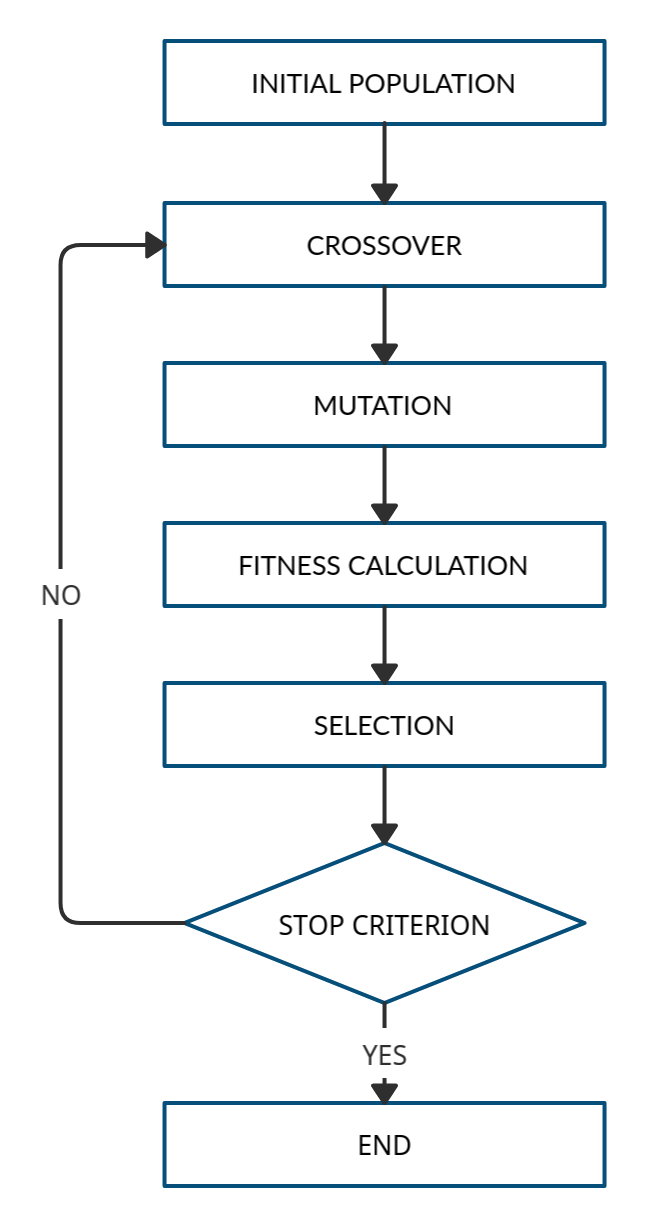
\includegraphics[scale=0.3]{img/GeneticAlg.png}
    \caption{Genetic algorithm structure.}
    \label{fig:GAlg}
\end{figure}

This algorithm is composed of different parts, all presented in the Figure \ref{fig:GAlg}. Each of this parts, except the initial population, are repeated until the stop criterion is satisfied. This stop criterion consists on whether the algorithm has performed an stablished number of iterations.


\subsubsection*{Initial population:}
The complete set of initial solutions or initial population is composed of two main groups. First, 60\% of the initial population are final solutions from the previously implemented GRASP algorithm, with the intention of stacking the GRASP algorithm and the Genetic algorithm (GA) in order to obtain better results. Second, the rest of the initial population (40\%) are randomized solutions.

These random solutions are composed of the same orders of the proposed problem but assigning each order a random warehouse. However, this warehouse must be one of the possible platforms to which the order can be assigned, thus complying with the limitations of the order.

Before starting the iterating part of the algorithm, the fitness of each solution is calculated, in order to execute the crossover part.

\subsubsection*{Crossover:}
Once the fitness of each solution from the population is obtained, the list of all solutions is sorted in ascending order, placing the solutions with better fitness at the first positions. A list composed of parent pairs is then formed by selecting the two best solutions that have not yet been assigned in order to form each parent pair.

The objetive of the crossover or reproduction is to obtain a number of new solutions (or children) from each parent pair. To achieve this goal, each child is formed by a random fraction of the orders that compose one of the parents, and the rest of the orders are taken from the remaining parent. The number of childs that are breeded is variable, and it is passed to the algorithm as a paramater. The result of this process is a list that contains sets of solutions called families, each one formed by a parent pair and a number of children.

\subsubsection*{Mutation:}
In order to avoid local minima during the finding of solutions that minimize the fitness function, the process of mutation is performed. This step of the algorithm is composed of two parts, and consists of randomly changing the assigned warehouses of a set of orders in a solution.

First, a random value is obtained for each member of a family.Then, this value is compared to a parameter $k$ in order to determine whether this member will mutate or not. Second, for each solution or member selected for mutating, 1\% of its orders are obtained, to which one of the possible warehouses will be assigned randomly.

\subsubsection*{Fitness calculation:}
The fitness value of every member of each family is calculated once the process of mutation is finished. This value is calculated by the fitness function.
This function takes into account the stock cost, the transport cost, and an alpha value that provides more weight to the transport cost.

\subsubsection*{Selection:}
Finally the new population or set of solutions is obtained taking into account the fitness value of every member of each family. This process uses a parameter value that stablishes the number of members of each family that will become part of the new population. The members selected are the ones with a better fitness value.

If the stop criterion is not satisfied, the algorithm iterates again starting in the crossover layer. If, on the contrary, this criterion is satisfied, the algorithm stops and keeps as final solution the member of the final population with the best fitness value. The criterion consists on a fixed number of iterations.
\section*{Evaluation}




\section*{Conclusions and future work}


Transport companies need to optimize their logistics infrastructures and strategies in order to be more efficient in a more competitive world. This work tries to merge two different problems, the warehouse stock management problem and the routing problem in order to minimize both the negative stock and the transport cost. To do this, a GRASP-based metaheuristic has been developed to improve the greedy algorithm that is currently being used by the company. The results in several case studies show that the greedy algorithm had a better behavior in the transport cost, since it is specially guided by a heuristic. However, the proposed GRASP algorithm overcomes the results obtained by the greedy algorithm in stock balancing, improving the negative average stock by up to 82\%.

In future works, we will improve the proposed algorithm by combining the proposed GRASP algorithm with a genetic algorithm (GA). Thus, the solutions obtained by the GRASP algorithm will participate as a subset of the initial population for the genetic algorithm. This could improve the quality of the solutions due to the high capability of the GA to combine previous solutions and avoid blockage in the local optimal.


\subsection*{Acknowledgements}
The paper has been partially supported by the Spanish research project TIN2016-80856-R.

\bibliography{bib}
\bibliographystyle{aaai}
\end{document}
